\section{Random Walks on Graphs}

\hyperdef{page}{rank}{Random walks on graphs arise in all sorts of
  applications.  One interesting example is Google and page rank, which
  we'll explore in this section.}

The hyperlink structure of the World Wide Web can be described as a
digraph. The nodes are the web pages or web-accessible files.  There is a
directed edge from node $x$ to node $y$ if the page associated with $x$
has a link to the page associated with $y$.  For example, in the following
graph the vertices $x_1, \ldots, x_n$ correspond to web pages and
$\diredge{x_i}{x_j}$ is a directed edge when page $x_i$ contains a
hyperlink to page $x_j$.

\mfigure{!}{2in}{figures/randomWalkFigs/webGraph}

The web graph is an enormous graph with many billions and probably even
trillions of nodes. At first glance, this graph wouldn't seem to be very
interesting. But in 1995, two students at Stanford, Larry Page and Sergey
Brin realized that the structure of this graph could be very useful in
building a search engine.  Traditional document searching programs had
been around for a long time and they worked in a fairly straightforward
way.  Basically, you would enter some search terms and the searching
program would return all documents containing those terms.  A relevance
score might also be returned for each document based on the frequency or
position that the search terms appeared in the document.  For example, if
the search term appeared in the title or appeared $100$ times in a
document, that document would get a higher score.  So if an author wanted
a document to get a higher score for certain keywords, he would put the
keywords in the title and make it appear in lots of places.  You can even
see this today with some bogus web sites.

This approach works fine if you only have a few documents that match a
search term.  But on the web, there are billions of documents and millions
of matches to a typical search.

For example, a few years ago a search on Google for ``math for computer
science notes'' gave 378,000 hits!  How does Google decide which 10 or 20
to show first?  It wouldn't be smart to pick a page that gets a high
keyword score because it has ``math math $\dots$ math'' across the front
of the document.

One way to get placed high on the list is to pay Google an advertising
fees ---and Google gets an enormous revenue stream from these fees.  Of
course an early listing is worth a fee only if an advertiser's target
audience is attracted to the listing.  But an audience does get attracted
to Google listings because its ranking method is really good at
determining the most important relevant web pages.  For example, Google
demonstrated its accuracy in our case by giving first rank to the Fall
2002 open courseware page for 6.042 \texttt{:-)} .  So how did Google know
to pick 6.042 to be first out of $378,000$?

Well back in 1995, Larry and Sergey got the idea to allow the digraph
structure of the web to determine which pages are likely to be the most
important.

\subsection{A First Crack at Page Rank}

Looking at the web graph, any idea which node/page might be the best to
rank $1$st?  Assume that all the pages match the search terms for now.
Well, intuitively, we should choose $x_2$, since lots of other pages point
to it.  This leads us to their first idea: try defining the \emph{page
  rank} of $x$ to be the number of links pointing to $x$, that is,
$\text{indegree}(x)$.  The idea is to think of web pages as voting for the
most important page ---the more votes, the better rank.

Of course, there are some problems with this idea. Suppose you wanted
to have your page get a high ranking.  One thing you could do is to
create lots of dummy pages with links to your page.

\mfigure{!}{1.5in}{figures/randomWalkFigs/dummy}

There is another problem ---a page could become unfairly influential by
having lots of links to other pages it wanted to hype.

\mfigure{!}{1.5in}{figures/randomWalkFigs/outDegree}

So this strategy for high ranking would amount to, ``vote early, vote
often,'' which is no good if you want to build a search engine that's
worth paying fees for.  So, admittedly, their original idea was not so
great.  It was better than nothing, but certainly not worth billions of
dollars.

\subsection{Random Walk on the Web Graph}

But then Sergey and Larry thought some more and came up with a couple of
improvements.  Instead of just counting the indegree of a node, they
considered the probability of being at each page after a long random walk
on the web graph.  In particular, they decided to model a user's web
experience as following each link on a page with uniform probability.
That is, they assigned each edge $x \rightarrow y$ of the web graph with a
probability conditioned on being on page $x$:
\[
\prcond{\text{follow link}\ \diredge{x}{y}}{ \text{at page $x$}} \eqdef
\frac{1}{\text{outdegree}(x)}.
\]
The user experience is then just a random walk on the web graph.

For example, if the user is at page $x$, and there are three links from
page $x$, then each link is followed with probability $1/3$.

We can also compute the probability of arriving at a particular page, $y$,
by summing over all edges pointing to $y$.  We thus have
\begin{eqnarray}
  \pr{\text{go to $y$}} &=&  \sum_{\text{edges}\ \diredge{x}{y}}
  \prcond{\text{follow link}\ \diredge{x}{y}}{\text{at page $x$}} \cdot
  \pr{\text{at page $x$}} \nonumber\\
  &=& \sum_{\text{edges}\ \diredge{x}{y}} \frac{\pr{\text{at
      $x$}}}{\text{outdegree}(x)} \label{LN12:stepprob}
\end{eqnarray}
For example, in our web graph, we have
\[ \pr{\text{go to $x_4$}} = \frac{\pr{\text{at $x_7$}}}{2} +
\frac{\pr{\text{at $x_2$}}}{1} \ .
\]
One can think of this equation as $x_7$ sending half its probability to
$x_2$ and the other half to $x_4$. The page $x_2$ sends all of its
probability to $x_4$.

There's one aspect of the web graph described thus far that doesn't mesh
with the user experience ---some pages have no hyperlinks out.  Under the
current model, the user cannot escape these pages.  In reality, however,
the user doesn't fall off the end of the web into a void of nothingness.
Instead, he restarts his web journey.

To model this aspect of the web, Sergey and Larry added a supernode to the
web graph and had every page with no hyperlinks point to it.  Moreover,
the supernode points to every other node in the graph, allowing you to
restart the walk from a random place.  For example, below left is a graph
and below right is the same graph after adding the supernode $x_{N+1}$.

\bigskip\centerline{
  \resizebox{!}{1.3in}{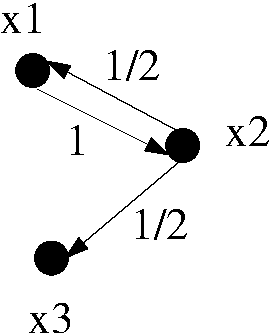
\includegraphics{figures/randomWalkFigs/adjMatrix2}}
  \hspace{2cm}
  \resizebox{!}{1.5in}{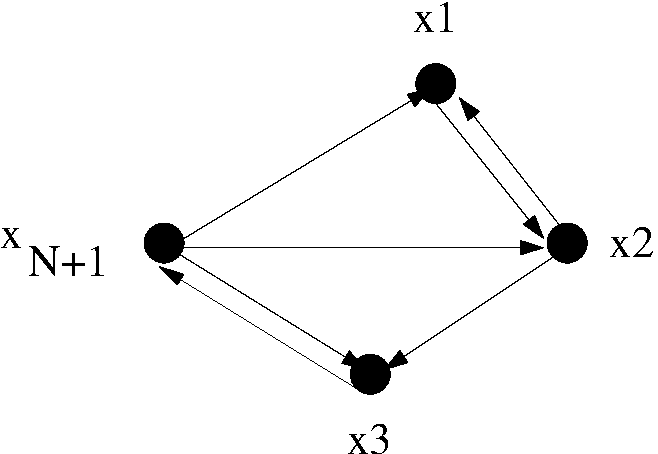
\includegraphics{figures/randomWalkFigs/sinkGraph}}
}\bigskip

The addition of the supernode also removes the possibility that the value
$1/\text{outdegree}(x)$ might involve a division by zero.

\subsection{Stationary Distribution \& Page Rank}

Page rank is basically just a stationary distribution over the web
graph (there are some more details, but this is the main idea), so
let's define a stationary distribution.

Suppose each node is assigned a probability that corresponds, intuitively,
to the likelihood that a random walker is at that node at a randomly
chosen time.  We assume that the walk never leaves the nodes in the graph,
so we require that
\begin{equation}\label{LN12:sum1}
\sum_{\text{nodes}\ x} \pr{\text{at $x$}} = 1.
\end{equation}

\begin{definition} An assignment of probabililties to nodes in a digraph
  is a \term{stationary distribution} if for all nodes $x$
\[
\pr{\text{at $x$}} = \pr{\text{go to $x$ at next step}}
\]
\end{definition}  

Sergey and Larry defined their page ranks to be a stationary distribution
They did this by solving the following system of linear equations: find a
nonnegative number, $\text{PR}(x)$, for each node, $x$, such that
\begin{equation}\label{LN12:PReqs}
\text{PR}(x) = \sum_{\text{edges}\ \diredge{y}{x}} \frac{\text{PR}(y)}{\text{outdegree}(y)},
\end{equation}
corresponding to the intuitive equations given in \eqref{LN12:stepprob}.  These
numbers must also satisfy the additional constraint corresponding
to~\eqref{LN12:sum1}:
\begin{equation}\label{LN12:sum1PR}
\sum_{\text{nodes}\ x} \text{PR}(x) = 1.
\end{equation}
So if there are $n$ nodes, then equations~\eqref{LN12:PReqs} and~\eqref{LN12:sum1PR}
provide a system of $n+1$ linear equations in the $n$ variables,
$\text{PR}(x)$.  Note that constraint~\eqref{LN12:sum1PR} is needed because the
remaining constraints~\eqref{LN12:PReqs} could be satisfied by letting
$\text{PR}(x)\eqdef 0$ for all $x$, which is useless.

Sergey and Larry were smart fellows, and they set up their page rank
algorithm so it would always have a meaningful solution.  Their addition
of a supernode ensures there is always a \emph{unique} stationary
distribution.  Moreover, starting from \emph{any} node and taking a
sufficiently long random walk on the graph, the probability of being at
each page will get closer and closer to the stationary distribution.  Note
that general digraphs without supernodes may have neither of these
properties: there may not be a unique stationary distribution, and even
when there is, there may be starting points from which the probabilities
of positions during a random walk do not converge to the stationary
distribution.  

\iffalse

\begin{optional}
Here's a note on solving the system of linear constraints, for the
interested reader.

Let $W$ be the $n \times n$ with the entry $w_{ij}$ (in row $i$ and
column $j$) having the value $w_{ij} = 1/\text{outdegree}(x_i)$ if edge
$x_i \rightarrow x_j$ exists, and $w_{ij} = 0$ otherwise.  For example, in
our last example with the 4-node graph (including the supernode), we have
$W$ given by:
\[
\left( \begin{array}{cccc}
    0 & 1 & 0 & 0 \\
    \frac{1}{2} & 0 & \frac{1}{2} & 0 \\
    0 & 0 & 0 & 1\\
    \frac{1}{3} & \frac{1}{3} & \frac{1}{3} & 0 \end{array} \right)
\]

The system of linear equations can now be described by a single matrix
vector product equation $W^T \vec{P} = \vec{P}$, where $W^T$ denotes the
transpose of $W$, and $\vec{P}$ is the column vector of page probabilities
(ranks):
\[\vec{P}\eqdef
\left( \begin{array}{c}
    \text{PR}(x_1) \\
    \text{PR}(x_2) \\
    \vdots \\
    \text{PR}(x_n) \end{array} \right)
\]
So the $j$th entry of the solultion vector, $\vec{P}$, is
\[
\sum_{1\leq i \leq n} w_{ij} \cdot \text{PR}(x_i) =
\sum_{i \mid x_i \rightarrow x_j} \frac{\text{PR}(x_i)}{\text{outdegree}(x_i)},
\]
which is exactly the constraint corresponding to node $x_j$
in~\eqref{LN12:PReqs}.

If you have taken a linear algebra or numerical analysis course, you
realize that the vector of page ranks is just the \emph{principle
  eigenvector} of the matrix, $W$, of the web graph!  Once you've had such
a course, these values are easy to compute.  Of course, when you are
dealing with matrices of this size, the problem gets a little more
interesting.
\end{optional}
\fi

Now just keeping track of the digraph whose nodes are billions of web
pages is a daunting task.  That's why Google is building power plants.
Indeed, Larry and Sergey named their system Google after the number
$10^{100}$ ---which called a ``googol'' ---to reflect the fact that the
web graph is so enormous.

Anyway, now you can see how 6.042 ranked first out of 378,000 matches.
Lots of other universities used our notes and presumably have links to the
6.042 open courseware site, and the university sites themselves are
legitimate, which ultimately leads to 6.042 getting a high page rank in
the web graph.

\endinput